\chapter{Análise dos casos de estudo}

A presente seção visa relatar casos reais de empresas que vivenciaram os estilos arquiteturais
estudados, optando em algum momento por fazer a migração de uma arquitetura monolítica para uma
arquitetura de microsserviços ou vice-versa. A proposta é detalhar e entender o contexto dessas empresas,
as decisões tomadas e qual a percepção que elas obtiveram sobre seus sistemas ao experimentar diferentes
arquiteturas.

Serão abordados quatro casos:

\begin{enumerate}
    \item \textbf{KN Login:} um monolítico legado transformado em uma série de sistemas
        autocontidos, com o intuito de caminhar em direção a uma arquitetura de microsserviços;
    \item \textbf{Otto:} a reimplementação do zero de um monolítico em uma arquitetura de sistemas
        autocontidos que posteriormente é evoluída para microsserviços;
    \item \textbf{Segment}: a transição de um monolítico para uma arquitetura de microsserviços,
        seguido do retorno para a arquitetura monolítica após as várias dificuldades encontradas;
    \item \textbf{RuaDois}: a adoção de uma arquitetura de microsserviços por uma \textit{startup}
        logo no início do sistema e a sua transição para uma arquitetura de monolítica.
\end{enumerate}

\section{KN Login}
\label{sec:KNLogin}

O caso apresentado nessa seção é um relato de \citeonline{Olga2016:SelfContainedSystems} a respeito
da transição realizada por Björn Kimminich\footnote{Gerente sênior de arquitetura de TI na empresa
Kuehne + Nagel. Mais informações em: \url{https://www.linkedin.com/in/bkimminich}} e sua equipe na empresa
Kuehne + Nagel\footnote{Vide \url{https://home.kuehne-nagel.com}} de um sistema monolítico para sistemas
auto-contidos\footnote{O relato original e completo da autora sobre o caso pode ser encontrado no link
\url{https://www.elastic.io/breaking-down-monolith-microservices-and-self-contained-systems/}}. 

A Kuehne + Nagel é uma empresa especializada em transportes e logística que presta serviços em uma
escala global. Dentre as aplicações de software utilizadas na empresa para entrega dos seus
produtos, existe um serviço chamado KN Login, o qual proporciona diversas funcionalidades
importantes para a empresa, como gerenciamento dos contêineres transportados, auxilia no controle da
integridade e eficiência da cadeia de suprimentos de seus clientes, rastreio dos contêineres com
análise das condições ambientais, etc.

\subsection{Problemática da aplicação}

O KN Login é um sistema monolítico iniciado em 2007 construído em cima do \textit{framework}
Java Web\footnote{Vide \url{https://docs.oracle.com/javase/7/docs/technotes/guides/javaws/developersguide/overview.html}}.
Inicialmente foi construído como uma aplicação simples mas com o passar do tempo se tornou um imenso
monolítico com mais de um milhão de linhas de código e com uma grande variedade de atribuições e
responsabilidades dentro da empresa. Esse contexto trouxe a equipe de software da Kuehne + Nagel as
seguintes dificuldades:

\begin{itemize}
    \item A impossibilidade de trocar o \textit{framework} Java Web para outra tecnologia que se
        adeque melhor as necessidades da empresa, uma vez que o \textit{framework} se encontra enraizado no sistema;
    \item A manutenção de dois \textit{frameworks} em paralelo na mesma aplicação, visto que, a
    equipe de \gls{TI} deles recomenda o uso do Spring Framework\footnote{Vide \url{https://spring.io}} em
    detrimento do Java Web Framework sempre que possível;
    \item Várias tecnologias diferentes de \gls{UI} utilizadas para conseguir atender as diferentes
    problemáticas enfrentadas pela empresa;
    \item O sistema se tornou bastante instável mediante a vasta variedade de tecnologias aplicadas,
    tornando difícil a manutenção do mesmo pela equipe;
    \item Alta complexidade que dificulta a entrada de novos membros no time de desenvolvimento.
\end{itemize}

\subsection{Solução adotada}

Mediante as dificuldades enfrentadas, a Kuehne + Nagel optou por seguir os seguintes passos:

\begin{itemize}
    \item Parar de adicionar quaisquer funcionalidades ou modificações no sistema por mais
        importante que estas sejam para o escopo do negócio;
    \item Identificar os módulos e limites do monolítico, de forma que fosse possível criar uma
        separação ou até mesmo cortar tais partes do monolítico;
    \item Ter ciência de quão dependentes são cada módulo dentro do monolítico, de tal forma que
        alguns sejam aparentemente impossíveis de separar;
    \item Começar a separação de cada módulo aos poucos, de maneira que pedaços possam ser
        desativados no monolítico a medida que cada novo módulo é liberado;
\end{itemize}

Após analisar esses quatro fatores, a equipe técnica da Kuehne + Nagel chegou ao ponto de que a
mudança diretamente para microsserviços seria inviável mediante a grande complexidade do monolítico,
além de que esta mudança não iria contribuir para deixar mais fácil a visualização que eles
tinham do sistema. Diante desta situação a equipe optou por abordar uma arquitetura de sistemas
autocontidos\footnote{Abordagem arquitetural que consiste em quebrar o sistema em vários sistemas
independentes, cada um com sua propría \gls{UI}, camada de lógica e persistência de dados.}.

Sistemas autocontidos segundo \citeonline{Olga2016:SelfContainedSystems}, diference dos
microsserviços por serem aplicações web autônomas e substituíveis as quais tendem a ser maiores do
que um microsserviço e possuem uma unidade de \gls{UI} própria. Assim, a Kuehne + Nagel construiu o
seu primeiro sistema autocontido chamado KN Freightnet, o qual contou com a duplicação de algumas
funcionalidades presentes no KN Login, representando o primeiro passo para minimizar a complexidade
do KN Login.

\subsection{Panorama pós-adoção da solução}

O relato apresentado por \citeonline{Olga2016:SelfContainedSystems}, não traz informações a respeito
de quais foram os resultados efetivos da adoção de sistemas autocontidos mediante as dificuldades
que a equipe enfrentava dentro no monolítico KN Login, mas a autora traz a perspectiva de utilizar
sistemas autocontidos como um passo intermediário em direção aos microsserviços quando o monolítico
em mãos tem uma complexidade muito alta para ser quebrado.

\subsection{Análise sobre o caso de estudo}

O caso da KN Login traz a típica história dos monolíticos: inicialmente uma aplicação que deveria
ser simples mas que com o tempo o sistema foi inflando com várias funcionalidades. Nota-se que a
equipe do KN Login se deparou com um contexto complexo: rastreio dos contêineres, análise climática,
etc. E mediante esse contexto, eles tentaram lidar com toda a problemática dentro do monolítico sem
considerar a limitação que este estilo arquitetural oferece referente a heterogeneidade das
tecnologias envolvidas.

Diante da combinação: contexto complexo e heterogeneidade de tecnologias, o monolítico KN Login
resultou em uma aplicação de alta complexidade e baixa confiabilidade, se tornando um sistema
instável e difícil de manter. A \autoref{fig:monoKN} visa ilustrar os pontos destacados na
arquitetura monolítica do KN Login mediante aos fatores levantados sobre essa arquitetura na
\autoref{monoSintese}. 

\begin{figure}[h]
  \centering
  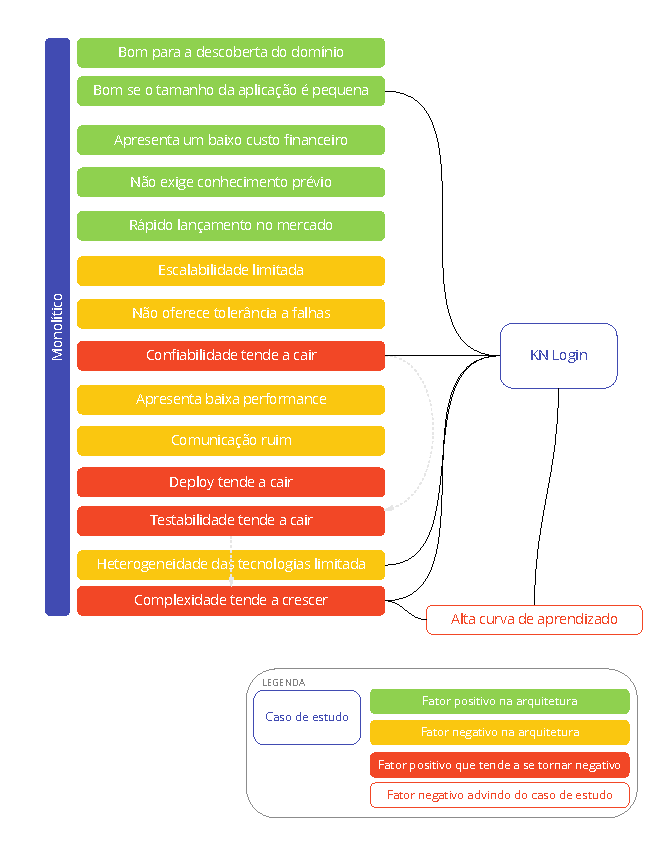
\includegraphics[keepaspectratio=true,scale=1]{figuras/analise-knlogin.eps}
  \caption{Fatores apresentados no caso de estudo da arquitetura monolítica do sistema KN Login\label{fig:monoKN}}
\end{figure}

\section{Otto}

Nesta seção será apresentado o caso relatado por  \citeonline{Guido2015:OnMonolithsAndMicrosrvices}, a
respeito da construção do novo \textit{e-commerce} Otto\footnote{O relato original e completo do autor
sobre o caso pode ser encontrado nos links
\url{https://www.otto.de/jobs/technology/techblog/artikel/on-monoliths-and-microservices_2015-09-30.php}
e \url{https://www.otto.de/jobs/technology/techblog/artikel/why-microservices_2016-03-20.php}}.O Grupo
Otto\footnote{Vide: \url{https://www.otto.de}} é uma empresa de origem alemã que trabalha em diversos países
desenvolvendo soluções de negócios voltadas a necessidade do setor de \textit{e-commerce}.

\subsection{Problemática da aplicação}

O sistema da Otto originou-se inicialmente em um projeto que deveria ser simples, no qual
implicitamente a equipe adotou uma macroarquitetura monolítica sem considerar ou até mesmo enxergar
que tal decisão estava sendo tomada. E mediante tal decisão, a equipe passou a ter dificuldades
com os problemas apresentados abaixo:

\begin{itemize}
    \item Escalabilidade limitada ao balanceamento de carga;
    \item Dificuldade de manutenção crescia juntamente com o crescimento da aplicação;
    \item Dificuldade de contratar desenvolvedores dispostos a trabalhar em um sistema de alta
        complexidade;
    \item Dificuldades ao realizar o \textit{deploy} principalmente no caso de aplicações sem
        períodos de inatividade;
    \item Dificuldades para trabalhar com várias equipes diferentes em uma mesma aplicação.
\end{itemize}

\citeonline{Guido2015:OnMonolithsAndMicrosrvices} enfatiza três pontos que para ele são importantes:

\begin{itemize}
    \item O desenvolvimento começa em equipe e no início a aplicação é bastante compreensível,
        necessitando apenas de uma única aplicação;
    \item Quando se tem um único aplicativo, o custo inicial é relativamente baixo: construção do
        repositório, automatização da \textit{build} e do processo de \textit{deploy}, configurar
        ferramentas de monitoramento, etc. Ativar e operar um novo aplicativo é relativamente fácil;
    \item É mais complexo operar grandes sistemas distribuídos do que um \textit{cluster}
        balanceador de carga.
\end{itemize}

\subsection{Solução adotada}

Diante do contexto apresentado, a Otto decidiu por começar um novo sistema de \textit{e-commerce},
adotando dessa vez uma arquitetura semelhante a apresentada na \autoref{sec:KNLogin} de sistemas autocontidos. Para
tal, eles estabeleceram quatro equipes funcionais dando origem a quatro aplicações. Os custos
iniciais de cada aplicação foram minimizados padronizando o processo de automação.

A medida que o sistema da Otto evoluía foram criados novos sistemas autocontidos, cada um com sua própria equipe
de desenvolvimento, seu próprio \textit{frontend} e seu próprio
banco de dados, tudo dentro de um escopo de negócio muito bem definido a respeito das suas
atribuições.

A Otto definiu aspectos macro e microarquiteturais. Os aspectos
microarquiteturais estavam voltados ao contexto local de cada sistema autocontido construído,
enquanto que nos aspectos macro foram definidos questões mais globais a respeito da arquitetura, como por exemplo:

\begin{itemize}
    \item A comunicação entre os sistemas autocotidos deveria ser feita sempre por meio do modelo
        \gls{REST};
    \item Não poderia existir estado mutável compartilhado entre as aplicações;
    \item Os dados devem ser compartilhados por meio de uma \gls{API} \gls{REST}, havendo somente
        uma aplicação responsável pelo dado e as outras unicamente com a permissão de leitura sobre o
        mesmo.
\end{itemize}

Nessa abordagem arquitetural escolhida, a Otto se deparou com dificuldades no compartilhamento
de dados entre as aplicações, o que os levou a adotar a estratégia de replicação de dados, na qual,
eventualmente eles precisam lidar com inconsistências temporárias entre os sistemas.

Contudo, alguns sistemas autocontidos ficaram bastante volumosos após cerca de três anos trabalhando
em cima dessa arquitetura. Essa nova situação fez com que a Otto adota-se uma nova medida em direção
a uma arquitetura de microsserviços. Decisão esta que segundo \citeonline{Guido2016:WhyMicroservices}
não gerou um processo tão árduo dentro da empresa uma vez que eles já vinham trabalhando em cima de
uma arquitetura bastante modularizada e já trabalhavam de forma concisa as questões de limites de
cada aplicação.

\subsection{Panorama pós-adoção da solução}

Após a adoção de uma arquitetura autocontida e a migração para uma arquitetura de microsserviços,
\citeonline{Guido2016:WhyMicroservices} traz como pontos positivos de ambas as arquiteturas os
seguintes pontos:

\begin{itemize}
    \item Facilidade em estabelecer uma pirâmide de testes que funcione de forma eficiente e rápida,
        auxiliando os desenvolvedores no lançamento de novas versões do código;
    \item Facilidade em gerenciar e integrar o trabalho de diferentes equipes uma vez que cada uma
        está trabalhando em seu próprio serviço;
    \item Aumento na velocidade de implantação de novas funcionalidades, sendo mais fácil testar e
        coletar rapidamente \textit{feedback};
    \item Cada aplicativo pode ser implementado de forma independente;
    \item Não há necessidade de coordenar o processo de implantação, cada equipe possui autonomia
        para gerenciar o seu processo de implantação sem afetar as demais equipes;
    \item Baixa curva de aprendizado, cada serviço é de fácil compreensão pelos desenvolvedores;
    \item Escalabilidade em relação a aplicação e aos próprios times de desenvolvimento;
    \item A complexidade de um serviço é extremamente baixa quando comparada a uma arquitetura
        monolítica;
    \item O sistema não está limitado a uma tecnologia específica;
    \item Exige que todos os processo estejam automatizados;
    \item Facilidade em reverter a versão do projeto quando algum \textit{bug} é introduzido;
    \item A ocorrência de falhas não afeta o sistema por inteiro, somente uma parte dele;
    \item Permite manter com facilidade a alta coesão e o baixo acoplamento do sistema;
\end{itemize}

Segundo a visão do autor, os microserviços possibilitam a construção de um sistema de software muito
mais sustentável ao longo dos anos do que um sistema monolítico, de forma que nessa arquitetura é
possível substituir pequenos pedaços da aplicação quando for necessário, enquanto que em sistemas
monolíticos essa abordagem se torna muito mais complexa.

A adoção de sistemas autocontidos é apresentada por ele como uma porta de entrada na qual é possível
resolver problemas semelhante aos microsserviços de uma forma mais pragmática, deixando ainda a
possibilidade de migrar futuramente para uma arquitetura de microsserviços de uma forma não tão
árdua \cite{Guido2016:WhyMicroservices}.
    
\subsection{Análise sobre o caso de estudo}

A \autoref{fig:analise-mono-otto} ilustra os pontos da arquitetura monolítica levantados pelo
caso de estudo da Otto. Percebe-se que a experiência deles atesta os pontos referentes ao início do
projeto quando a aplicação é pequena, de fácil compreensão por todos, tem um custo baixo, etc.
Também atesta os problemas de complexidade e de implantação que tendem nesse modelo arquitetural a
crescer juntamente com a base de código.


\begin{figure}[h]
  \centering
  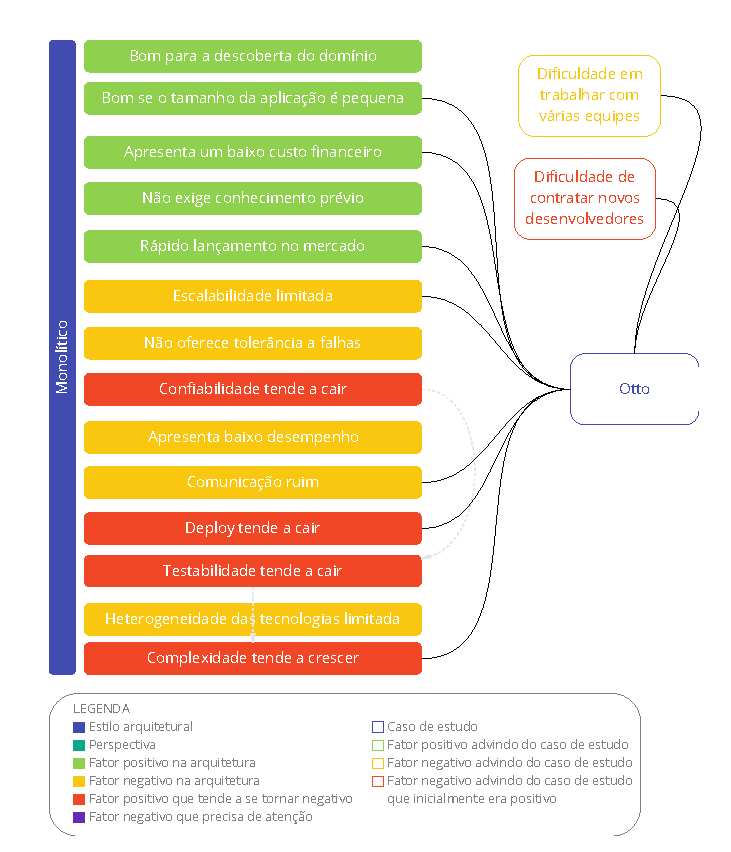
\includegraphics[keepaspectratio=true,scale=1]{figuras/monoOtto.eps}
  \caption{Fatores apresentados no caso de estudo da arquitetura monolítica da Otto\label{fig:analise-mono-otto}}
\end{figure}

A tomada de decisão por migrar para uma arquitetura de sistemas auto-contidos auxilia eles como um
passo intermediário antes de aderir toda a complexidade da arquitetura de microsserviços. Nessa
abordagem percebe-se que eles vivenciam características dos dois estilos arquiteturais. Olhando da
perspectiva dos microsserviços, eles definem protocolos de comunicação e compartilhamento de dados e lidam
com eventuais inconsistência de dados (um problema comum da arquitetura de microsserviços). Por
outro lado, eles ainda precisam lidar com a crescente base de código dos monolíticos dentro de cada
sistema auto-contido.

A \autoref{fig:analise-micro-otto} ressalta os pontos da arquitetura de microsserviços
adotada pela Otto, na qual nota-se alta escalabilidade, alta tolerância a falhas, facilidade no
\textit{deploy}, testabilidade e alta heterogeneidade de tecnologias observados no caso de estudo.
A experiência da Otto também traz outros pontos dessa arquitetura, não presentes no mapa mental
construído, como baixa curva de aprendizado e a necessidade de automatizar todos os processos.  

Um ponto que se diferencia do esperado, de acordo com a fundamentação teórica levantada para esse
trabalho, é que a Otto apresenta a coleta de \textit{feedbacks} como um ponto positivo da
arquitetura de microsserviços enquanto o referencial teórico aponta a arquitetura monolítica como
mais indicada para tal. Nesse sentido, percebe-se que existe o fator tempo de projeto envolvido.
Como relatado na \autoref{Perspectivas:Problematica} e na \autoref{effortsAndTime}, ao iniciar um
projeto a arquitetura monolítica é melhor para a rápida coleta de \textit{feedbacks} por ser mais
simplista, contudo no caso da Otto, eles já tinham um sistema monolítico com uma base de código
grande e devido aos problemas de complexidade já discutidos evoluir e testar rápido esse sistema com
os usuários já não deveria ser um processo tão fácil. Já na arquitetura de microsserviços, existe o
esforço inicial de automatizar todos os processos e de planejar cuidadosamente os limites de domínio
de cada aplicação, mas após essas etapas estarem bem definidas alterar e testar novos serviços tende
a ser fácil.

\begin{figure}[h]
  \centering
  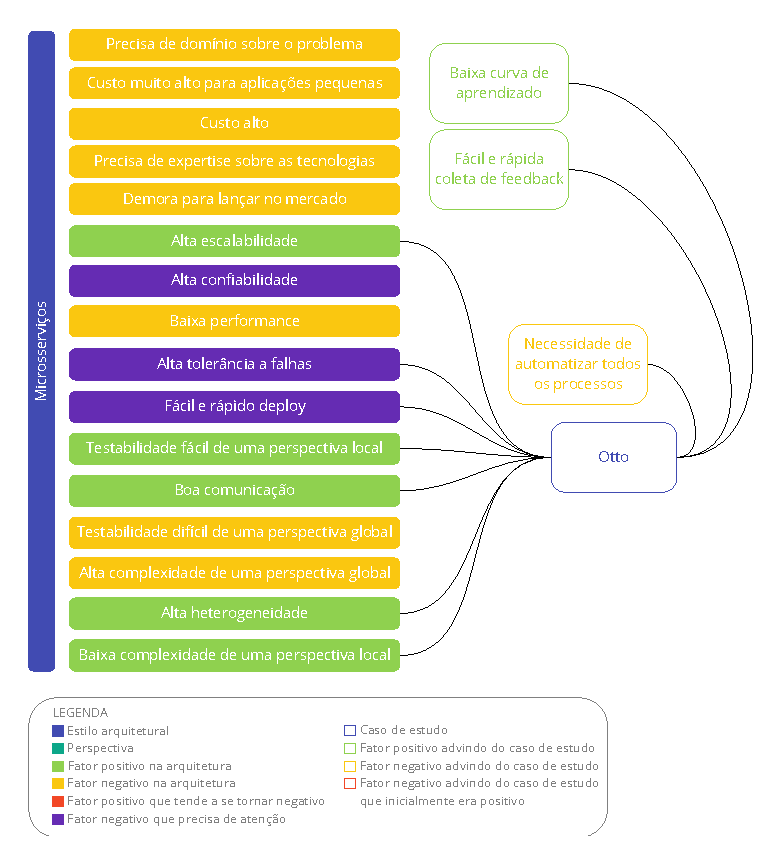
\includegraphics[keepaspectratio=true,scale=1]{figuras/analise-micro-otto.eps}
  \caption{Fatores apresentados no caso de estudo da arquitetura de microsserviços da Otto\label{fig:analise-micro-otto}}
\end{figure}

\section{Segment}

O caso apresentado a seguir foi retratado por \citeonline{Noonan:ToMicroservicesAndBackAgain} na
conferência QCon London. Ela trata a respeito do sistema da Segment\footnote{Vide:
\url{https://segment.com}}, o qual foi construído inicialmente em uma arquitetura monolítica,
passou por uma migração para uma arquitetura de microsserviços e após 3 anos em cima desta
arquitetura, decidiram por retornar para a arquitetura monolítica.

A Segment é uma empresa responsável por fazer a integração entre as aplicações de software de seus
clientes com diversas ferramentas de análise de dados, atuando como um \textit{pipeline} facilitador
na integração entre as partes citadas. 

\subsection{Problemática da aplicação}

Em 2013, quando a empresa foi criada havia necessidade de construir um sistema que possuísse uma
baixa sobrecarga operacional, sendo simples de gerenciar e fácil de iterar, assim, diante de tais
necessidades a primeira versão do sistema da Segment foi construído em cima de uma arquitetura monolítica.

A arquitetura inicial consistia em uma \gls{API} de entrada que recebia os dados enviados pelas aplicações dos
clientes da Segment, e colocava esses dados em uma fila de processamento. A partir deste ponto,
havia uma monolítico responsável por consumir a fila e enviar os dados para as aplicações de destino
(Google Analytics, Salesforce...). O consumo dessa fila ocorria no modelo \gls{FIFO}\footnote{Vide
\url{https://pt.wikipedia.org/wiki/FIFO}}. A dificuldade enfrentada pela equipe da Segment nessa
arquitetura estava na tentativa de reenviar algum dado quando por algum motivo a primeira tentativa
tinha falhado. De acordo com \citeonline{Noonan:ToMicroservicesAndBackAgain}, cerca de 10\% das
solicitações para as aplicações de destino falhavam e nesses casos, o monolítico fazia de 2 a 10
tentativas de reenvio.

Nessa abordagem, a Segment passou a enfrentar um bloqueio frontal na fila. Sempre que uma aplicação
de destino estava muito instável ou ficava fora do ar, o monolítico travava a fila tentando refazer
o envio, de forma que o problema se propagava: ao invés de ter uma integração X fora do ar, todas as
outras integrações também paravam de funcionar visto que a fila estava bloqueada.

Após um ano trabalhando em cima dessa arquitetura, o time de desenvolvimento da Segment decidiu por
mudar para uma arquitetura de microsserviços visando o isolamento do ambiente, de forma que
problemas com uma determinada integração não impactasse na outra. Para tal, eles segregaram cada
integração em um serviço próprio acompanhado de sua própria fila e adicionaram antes das filas um
roteador capaz de receber os dados da \gls{API} de entrada e direcioná-los para as filas necessárias.
Essa abordagem trouxe as seguintes vantagens para a Segment:

\begin{itemize}
    \item Diminui a necessidade de \textit{backup} da fila, uma vez que ao falhar uma aplicação de
        destino eles não precisam mais salvar a fila toda, mas somente a parte referente a
        integração problemática;
    \item A falha em uma aplicação de destino não afetava mais as outras integrações;
    \item Facilitou a inserção de novas aplicações de destino ao sistema da empresa, permitindo um
        desenvolvimento mais rápido;
    \item Facilidade em tratar as peculiaridades de cada integração dentro do seu próprio serviço,
        sem precisar compatibilizar os dados com todas as aplicações de uma única vez;
    \item Agregou a visibilidade de toda a pilha do processo, permitindo identificar mais facilmente
        as falhas e a qual serviço específico elas eram referentes.
\end{itemize}

Em 2016, a Segment possui 50 serviços integrando diferentes aplicações. Com o aumento na quantidade
de serviços para gerenciar eles começaram a ter algumas dificuldades, entre elas:

\begin{itemize}
    \item Não possuíam processos de \textit{build} e \textit{deploy} automatizados, o que acaba
        exigindo bastante tempo da equipe mediante a quantidade de serviços no ar;
    \item Cada sistema realizava diferentes tratamentos sobre o dado antes de enviar para a
        aplicação de destino e como cada cliente podia enviar os dados de diferentes formas, acabou
        se tornando árduo entender o que estava se passando dentro de cada serviço. Nesse caso, eles
        optaram por criar bibliotecas comuns entre os serviços para fazer tal tratamento.
        Inicialmente, isto se refletiu positivamente dentro da equipe, mas sem os processos de
        implantação automatizados, a atualização da versão das bibliotecas em cada serviço se tornou
        um problema de tal forma que eles passaram a preferir não corrigir um \textit{bug} dentro da
        biblioteca do que fazer a atualização;
    \item Administrar o escalonamento da arquitetura não era uma tarefa fácil. Alguns clientes
        geravam um tráfego de milhares de requisições por segundo, e frequentemente acontecia de
        algum desses clientes ativarem alguma integração com o intuito de experimentar, e apesar das regras
        automáticas de escalonamento e dimensionamento de recursos, o time de \gls{TI} da Segment
        não conseguia encontrar uma regra de escalabilidade que se adequasse bem ao contexto deles.
        Diante desse caso, eles pensaram em soluções de supervisionamento da arquitetura, manter
        sempre alguns trabalhadores mínimos, etc., mas chegaram a conclusão de que essas abordagens
        teriam um custo muito alto para a empresa;
    \item Mesmo com todas as dificuldades, eles continuavam adicionando cerca de três aplicações de
        destino por mês. O que tornava cada vez mais complexa a base de código e fazia a carga
        operacional, diante dos processos não automatizados, crescer linearmente ainda que o tamanho
        da equipe fosse constante;
    \item A empresa chegou a parar de desenvolver novas funcionalidades visto que a complexidade e a
        dificuldade para manter os microsserviços funcionando estava altíssima;
    \item A carga encaminhada dos clientes havia aumentado consideravelmente e eles ainda
        continuavam com o mesmo problema de limitação do tráfego pelo lado das aplicações de
        destino, o mesmo bloqueio frontal mencionado anteriormente;
\end{itemize}

\subsection{Solução adotada}

Em 2017, \citeonline{Noonan:ToMicroservicesAndBackAgain} relata que eles chegaram ao ponto de
ruptura: haviam 140 serviços rodando, uma equipe pequena mantendo uma série de processos
operacionais e uma base de código complexa fazendo com que a arquitetura que inicialmente parecia
ideal e que os auxiliaria a escalar, se torna-se o fator paralisador de todo o sistema. Nesse ponto,
eles reuniram todas as experiências que haviam adquirido desde 2013, e tomaram a decisão de retornar
para uma arquitetura monolítica, com um sistema único que eles fossem capaz de gerenciar e escalar.

A solução adotada reuniu todas as 140 integrações no mesmo repositório novamente, ao invés de ter
uma fila para cada aplicação eles optaram por salvar os dados em um banco MySQL\footnote{Vide
\url{https://www.mysql.com}}, com as condições de que:

\begin{itemize}
    \item As linhas do banco deveriam ser imutáveis, devendo o monolítico sempre inserir o novo
        estado mas nunca atualizar o antigo;
    \item Operações de JOIN não deveriam ser realizadas. No modelo desenvolvido por eles, o
        monolítico deveria apenas ler informações básicas sobre os dados a serem tratados;
    \item A escrita deve ser a operação predominante. Nessa nova arquitetura, a maioria dos dados
        eram tratados em cache e tinham apenas o seu estado registrado no banco de dados.
\end{itemize}

Dessa forma, os dados chegavam ao monolítico, o qual registrava os mesmos no banco mas ainda os
mantinham em cache. A medida que os dados eram tratados, o monolítico removia os dados do cache e
registrava o novo estado no banco. Quando alguma integração falhava, o estado de falha era
registrado no banco para que fosse tratado posteriormente por meio da estratégia de \textit{backoff}
definida por eles.

Olhando a perspectiva da escalabilidade, o monolítico podia ser replicado sempre que houvesse a
necessidade. Para tal, havia um serviço responsável por gerenciar as instâncias de banco de dados.
Sempre que um novo monolítico era colocado no ar, ele recebia por meio desse serviço o acesso a um
banco de dados exclusivamente seu. Dessa forma, eles conseguiram automatizar o processo de
escalabilidade de acordo com o uso da CPU \cite{Segment2018:Centrifuge}\footnote{A descrição
completa da solução adotada pela Segment pode ser encontrada no link \url{https://segment.com/blog/introducing-centrifuge/}}.

\subsection{Panorama pós-adoção da solução}

A solução adotada pela Segment permitiu a eles:

\begin{itemize}
    \item Escalar melhor a sua aplicação, lidando de forma mais eficiente com as limitações de
        capacidade das aplicações destino e permitindo a adição de novos serviços sem a necessidade
        de aumentar os custos operacionais da equipe;
    \item Aumentou consideravelmente a produtividade do time;
    \item Solucionou o problema de compatibilidade de diferentes versões de bibliotecas
        compartilhadas entre os serviços;
    \item Facilitou o desenvolvimento de novas funcionalidades para o sistema;
\end{itemize}

Os problemas que eles tinham na primeira arquitetura monolítica relacionados às dificuldades de
isolamento de ambiente continuaram presentes nessa nova arquitetura, contudo, agora o time de
desenvolvimento da Segment soube lidar de forma muito mais madura com essa situação, procurando
outras soluções diferente de microsserviços para tratar os obstáculos com os quais eles se
deparavam.

\subsection{Análise sobre o caso de estudo}

O caso da Segment conta com três fases que precisam ser avaliadas: o monolítico inicial, os
microsserviços e o monolítico final. A \autoref{fig:analise-mono-segment-1} representa o
primeiro monolítico construído pela empresa. A escolha inicial de uma arquitetura monolítica condiz
com o contexto da empresa, a qual era composta por uma equipe pequena de engenheiros de software e
estava buscando validar sua ideia e descobrir o domínio no qual estavam imersos. 

\begin{figure}[h]
  \centering
  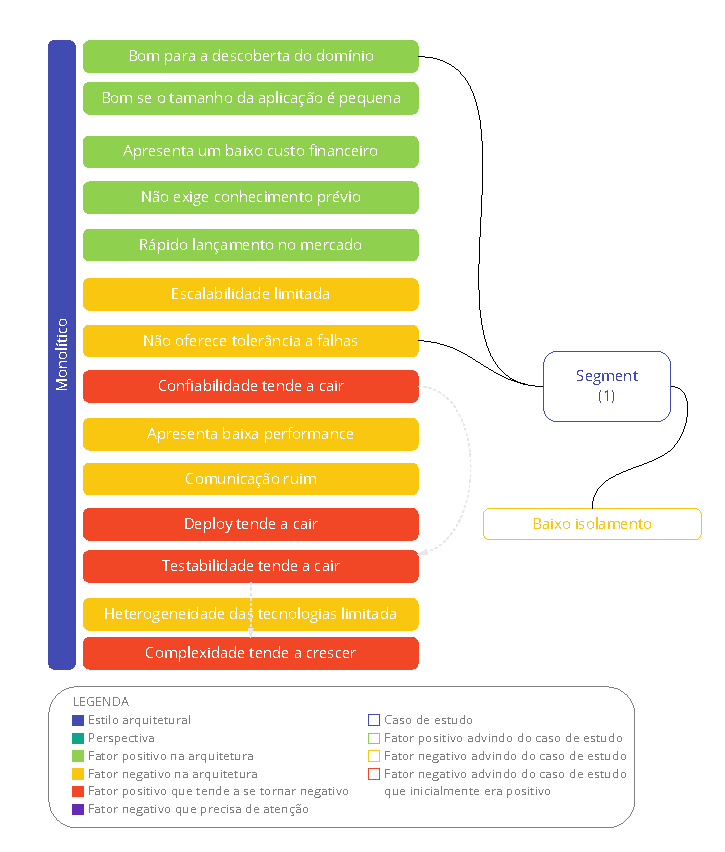
\includegraphics[keepaspectratio=true,scale=1]{figuras/analise-mono-segment-1.eps}
  \caption{Fatores apresentados no caso de estudo da primeira arquitetura monolítica da Segment\label{fig:analise-mono-segment-1}}
\end{figure}

No caso, a Segment se depara logo com a limitação de tolerância a falhas dessa arquitetura e decidem
mudar para uma arquitetura de microsserviços. Visto que o sistema da Segment era um software novo,
com um ano de funcionamento quando eles optaram por fazer a migração, percebe-se que outros problemas
da arquitetura monolítica não aparecem no relato, como alta complexidade, dificuldades de
manutenibilidade, etc., evidenciando o ponto levantado na \autoref{monoSintese} de que essas
características são inicialmente positivas no sistema e estão diretamente relacionadas ao tamanho da
base de código.

Ao passar o sistema para a arquitetura de microsserviços, o time consegue perceber os pontos
destacados na \autoref{fig:analise-micro-segment} como a tolerância a falhas, a baixa complexidade
local, etc. Vale ressaltar que a Segment também relata, semelhante a Otto, a facilidade e velocidade
de adicionar novas funcionalidades nessa arquitetura. Contudo, percebe-se também a ausência da expertise,
comentada na \autoref{Perspectivas:recursosHumanos}, sobre este modelo arquitetural visto que os processos
operacionais não são automatizados pela equipe da Segment. Este fator somado ao crescente número de
serviços funcionando faz com que a equipe se afogue na grande demanda de processos operacionais
exigida por essa arquitetura. Assim, eles param todo o desenvolvimento mediante a inviabilidade de
gerenciar essa arquitetura nas proporções que ela tomou.

\begin{figure}[h]
  \centering
  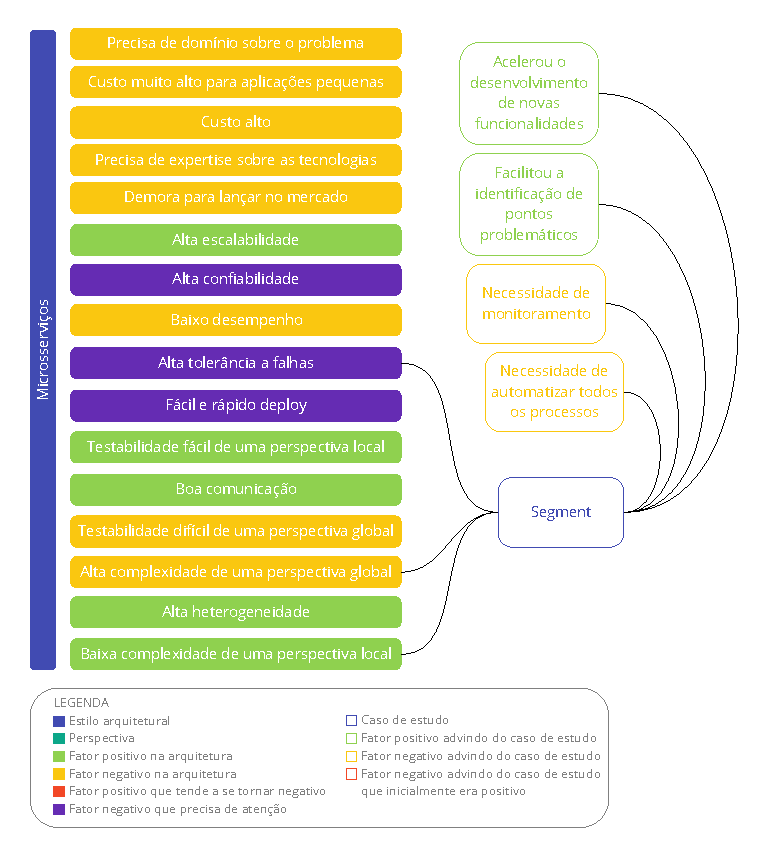
\includegraphics[keepaspectratio=true,scale=1]{figuras/analise-micro-segment.eps}
  \caption{Fatores apresentados no caso de estudo da arquitetura de microsserviços da Segment\label{fig:analise-micro-segment}}
\end{figure}

No meio desta situação, a Segment opta por voltar para a arquitetura monolítica mas de uma forma
mais consciente sobre quais eram as dificuldades do contexto deles, planejando estratégias para
lidar com as adversidades que eles já conheciam. Assim, eles conseguem construir um sistema que
possa prover escalabilidade, tolerância a falhas e produtividade para a equipe em cima de uma
arquitetura monolítica. Vale salientar que, a respeito da produtividade da equipe, a Segment se
encontra com um monolítico relativamente novo, que foi planejado e assim ele apresenta o perfil de
um monolítico em sua fase inicial: baixa complexidade, módulos bem definidos, etc., contudo, é
necessário que a equipe se empenhe para conseguir manter essas características a medida que sua base
de código cresce.

\section{RuaDois}

O caso apresentado nesta seção é o resultado de uma entrevista com Erlan Cassiano\footnote{Vide
\url{https://www.linkedin.com/in/erlan-cassiano-56370231/}}, \textit{Header of Product} da
\textit{startup} RuaDois\footnote{Vide \url{https://www.ruadois.com.br/pt-br/home}}, sobre a
experiência que eles passaram dentro da empresa ao iniciar com uma arquitetura de microsserviços
e optar por migrar para uma arquitetura monolítica. Este relato se diferencia dos outros casos
estudados, por ser uma migração na qual a presente autora deste documento fez parte do time de
desenvolvimento acompanhado de perto as dificuldades da equipe as quais trouxeram a inspiração para
realizar o presente estudo.

A RuaDois é uma empresa brasileira que surgiu em outubro de 2018 com o propósito de
solucionar as dificuldades enfrentadas tanto por parte das imobiliárias quanto por parte dos
locatários no processo de locação de imóveis. A proposta\footnote{Mais informações a respeito
da proposta e visão da RuaDois podem ser encontradas em
\url{https://open.spotify.com/episode/2jYKPCPLCIdDWwxpR0theT?si=dT6WUG7JSEGJH3mVVIJitQ}}
da empresa consiste em atuar como um facilitador para as imobiliárias
ingressarem no meio digital e consequentemente propiciar seu crescimento. Para tal,
eles buscam aumentar a eficiência do processo de locação por meio da digitalização,
proporcionando melhor integração entre operação e tecnologias. Assim, com um processo
mais digital, os recursos humanos podem ser melhores empregados no atendimento do
cliente favorecendo a experiência do mesmo nesse mercado tão burocrático.

\subsection{Problemática da aplicação}

O início do desenvolvimento do software da RuaDois se deu com o intuito de validar as ideias que
os fundadores tinham de melhorar a experiência dos locatários e da própria imobiliária com o processo
de visitação dos imóveis. O Cassiano relata que inicialmente eles construíram um \gls{MVP} visando
validar a ideia, e que naturalmente o desenvolvimento da aplicação caminhou para uma arquitetura de
microsserviços, composta neste começo por uma pequena aplicação \textit{frontend} denominada
\textit{widget}, algumas funções rodando em um modelo \textit{serverless}\footnote{Modelo de
execução no qual o provedor \textit{cloud} é responsável por realizar alocação dinâmica dos recursos
necessários para executar, em geral, as denominadas \gls{FaaS}.} e pelos serviços:

\begin{description}
    \item [\textit{r2service}] serviço responsável por gerenciar os imóveis e as propostas recebidas
        pelos imóveis;
    \item [\textit{r2visit}] serviço responsável por gerenciar as visitas aos imóveis.
\end{description}

O \textit{Header of product} da RuaDois conta que eles objetivavam com a arquitetura de
microsserviços obter maior estabilidade, independência entre os sistemas e maior tolerância a falhas,
principalmente em relação ao módulo de visitas visto que falhas nesse módulo geravam uma série de
problemas operacionais para as imobiliárias que utilizavam o sistema. Cassiano aponta os seguintes
pontos positivos que eles obtiveram nesse modelo arquitetural:

\begin{itemize}
    \item Facilidade em validar novas ideias dentro do escopo restrito de cada serviço;
    \item Facilidade e rapidez em realizar o \textit{deploy} de cada serviço;
    \item A possibilidade de testar diferentes abordagens de resolução do problema;
    \item A lógica interna de cada serviço podia ser alterada com facilidade.
\end{itemize}

Contudo, o time de desenvolvimento, composto naquele período por quatro membros, começou a enfrentar
algumas dificuldades, entre elas estão:

\begin{itemize}
    \item Um modelo rígido de comunicação foi definido entre os serviços, e mudar esses protocolos
        de comunicação garantindo a integração se tornou uma tarefa árdua; 
    \item Gerenciar cada serviço, chaves de integração, acesso ao banco, etc., era mais complicado
        tendo vários serviços separados;
    \item Evoluir os microsserviços com uma equipe pequena e com pouca experiência sobre o modelo
        arquitetural e tecnologias era difícil;
    \item A demanda inicial de clientes da \textit{startup} era baixa para justificar o custo de
        manter quatro instâncias dos serviços, contando ambiente de homologação, rodando sem
        consumir tantos recursos;
    \item Dificuldade em realizar testes de integração.
\end{itemize}

\subsection{Solução adotada}

Mediante a equipe pequena, as dificuldades encontradas e os custos de manter os serviços a equipe
técnica da RuaDois optou por migrar a arquitetura para um sistema monolítico, visando ganhar
testabilidade, confiabilidade e estabilidade nos módulos cuja a ideia base da solução já tinha sido
validada. Assim, eles optarem pela construção de um monolítico, contudo de forma modularizada
visando que no futuro pudesse ser simples a migração de volta para uma arquitetura de
microsserviços.

A primeira dificuldade da equipe foi a de convencer as outras áreas da empresa de que havia a
necessidade de migrar todo o sistema para uma arquitetura monolítica e quais seriam as vantagens
dessa arquitetura. Após a migração, que durou cerca de quatro meses, notaram-se as seguintes melhorias:

\begin{itemize}
    \item A base do código de \textit{backend} centralizada em um único lugar facilitou as
        dificuldades que haviam antes em relação a gerência dos microsserviços;
    \item Facilidade em testar todo o fluxo uma vez que todo o código se encontrava na mesma
        aplicação;
    \item Ganho de velocidade na evolução das funcionalidades já existentes;
    \item Ganho de estabilidade dos serviços;
\end{itemize}

Por outro lado, as seguintes dificuldades foram encontradas nesse modelo arquitetural:

\begin{itemize}
    \item Perda de velocidade na criação de novas funcionalidades;
    \item Ao fazer uma pequena alteração em determinada parte do sistema é necessário rodar a
        \textit{pipeline} inteira de teste tornando o processo de desenvolvimento mais lento;
    \item A dependência entre os módulos trazia a necessidade de alterar toda a aplicação para
        conseguir lançar algumas funcionalidades;
    \item Demandas pontuais da empresa, como a importação de XML que é executada apenas uma vez ao
        dia, consumiam muito da CPU e eles possuíam dificuldade para equilibrar custo e
        escalabilidade da instância de uma forma saudável para a empresa;
    \item Dificuldade de imersão de novos desenvolvedores, uma vez que havia a necessidade de
        compreender toda a base de código do monolítico;
    \item Demora reiniciar o monolítico quando acontece alguma falha no sistema;
    \item Estão limitados pela tecnologia. O monolítico foi construído usando do \textit{framework}
        Node.js\footnote{Vide \url{https://nodejs.org/}}, e atualmente eles desejam utilizar algumas
        bibliotecas do \textit{python} para processamento de imagens mas estão impossibilitados de
        fazer isso no monolítico;
    \item A limitação da tecnologia vale para o \textit{frontend} também, o qual foi construído em
        Vue.js\footnote{Vide \url{https://vuejs.org}}, mas eles desejam aplicar React\footnote{Vide
        \url{https://pt-br.reactjs.org}} em algumas partes do sistema que eles julgam mais adequado.
\end{itemize}

\subsection{Panorama pós-adoção da solução}

A visão do Erlan Cassiano após passar por ambos os estilos arquiteturais dentro da RuaDois é que
microsserviços são mais fáceis para validação de ideias uma vez que você é capaz de fechar os
escopos de cada serviço e testar diferentes abordagens para um mesmo problema sem precisar alterar na
aplicação inteira, tornando esse processo de validação e coleta de \textit{feedbacks} muito mais
rápido. Por outro lado, esse modelo arquitetural apresenta um custo alto de manutenção que não se
paga no início da empresa com poucos clientes. Na arquitetura monolítica o custo de manter esse
sistema é mais sustentável nos primeiros anos da \textit{startup}, contudo tende a crescer junto com
a camada de testes que é executada a cada \textit{deploy}, uma vez que as ferramentas de integração
contínua cobram por hora de execução.

Existe um ponto enfatizado por Cassiano que são os recursos humanos e como eles afetam a escolha da
arquitetura. Pelas experiências dele, microsserviços é um modelo arquitetural que exige mais conhecimento
e mais desenvolvedores compondo a empresa com o propósito de manter essa arquitetura funcionando bem.
Enquanto que a arquitetura monolítica se dá melhor com times pequenos contudo tende a ser mais difícil
quanto a inserção de novos desenvolvedores.

Por fim, ele relata que é essencial o sistema se adaptar aos objetivos de negócio e ao tempo da
empresa. Assim, ele sugere validar a ideia usando de serviços separados objetivando uma rápida coleta de
\textit{feedback}, após essa solução validada, estabilizar o sistema em uma arquitetura monolítica
visando ser financeiramente mais sustentável nesses primeiros anos da empresa, e por último avaliar
a mudança para uma arquitetura de microsserviços ou outro modelo arquitetural. Cassiano aponta este
como um caminho mais estratégico quando pensamos na evolução da \textit{startup}.

\subsection{Análise sobre o caso de estudo}

Diante do caso de estudo da RuaDois, percebe-se que, semelhante ao caso da Otto, eles afirmam que a
arquitetura de microsserviços é mais fácil para coletar \textit{feedbacks} dos clientes e testar
novas funcionalidades. Este é um reflexo da modularidade natural deste estilo arquitetural, que
torna fácil e rápida a concepção dos serviços de uma perspectiva local porém a RuaDois, nessa fase inicial
em que experimentaram essa arquitetura, possuía apenas dois serviços \textit{backends}, três
aplicações de \textit{frontend} (\textit{web}, \textit{mobile} e o \textit{widget}) e uma série de
funções \textit{serverless}, os quais não tinham ou apresentavam baixa automatização na maioria dos processos
de \textit{deploy} e integração contínua desses serviços. Assim percebe-se no relato uma dificuldade de
lidar com a gerência desses serviços quando olhamos para uma perspectiva mais global a respeito do caso.

O relato da RuaDois também enfatiza a importância do conhecimento sobre as tecnologias e sobre o
modelo arquitetural nessa abordagem de microsserviços, sendo fatores apresentados como fundamentais
para a evolução da mesma. A \autoref{fig:sintese-micro-ruadois} resume os pontos observados neste
estudo de caso.

\begin{figure}[h]
  \centering
  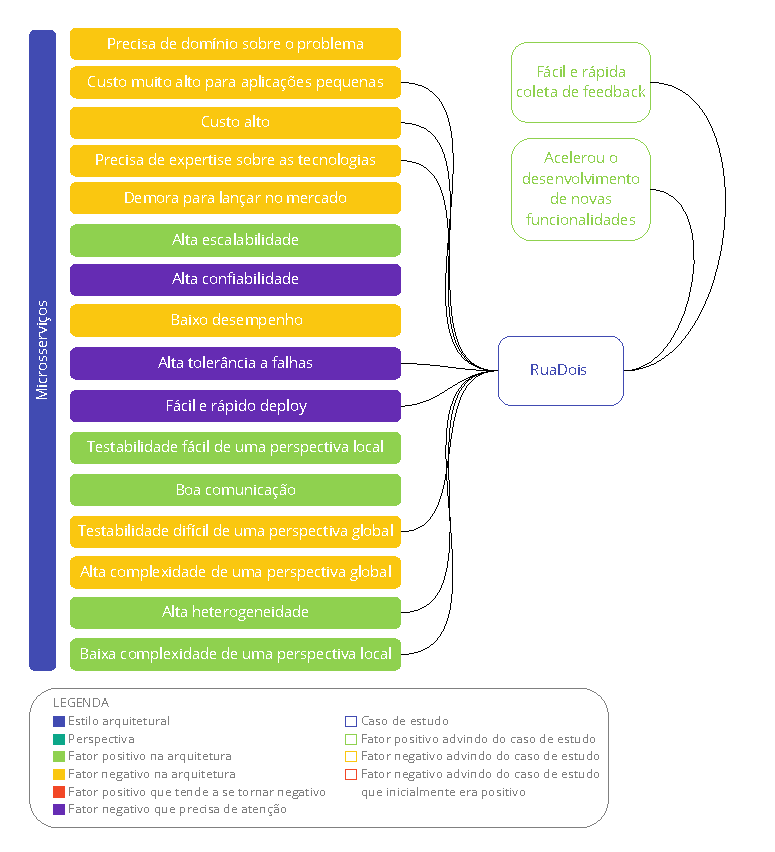
\includegraphics[keepaspectratio=true,scale=1]{figuras/analise-micro-ruadois.eps}
  \caption{Fatores apresentados no caso de estudo da arquitetura de microsserviços da RuaDois\label{fig:sintese-micro-ruadois}}
\end{figure}

Quando olhamos para a arquitetura monolítica da RuaDois, percebe-se que o custo da aplicação é mais
sustentável mediante o tamanho da empresa, também nota-se que a testabilidade do sistema por inteiro
é mais fácil visto que não há necessidade de integrar diferentes sistemas, entretanto essa testabilidade
posterga o processo de \textit{deploy} e gera um custo extra ao rodar um conjunto de testes que não estão
relacionados a funcionalidade alterada. Por fim, vemos que eles conseguem aumentar a estabilidade da
aplicação na arquitetura monolítica mas em contrapartida, a complexidade de desenvolver novas
funcionalidades nessa base acoplada tende a aumentar. A \autoref{fig:sintese-mono-ruadois} resume os
pontos observados.

\begin{figure}[h]
  \centering
  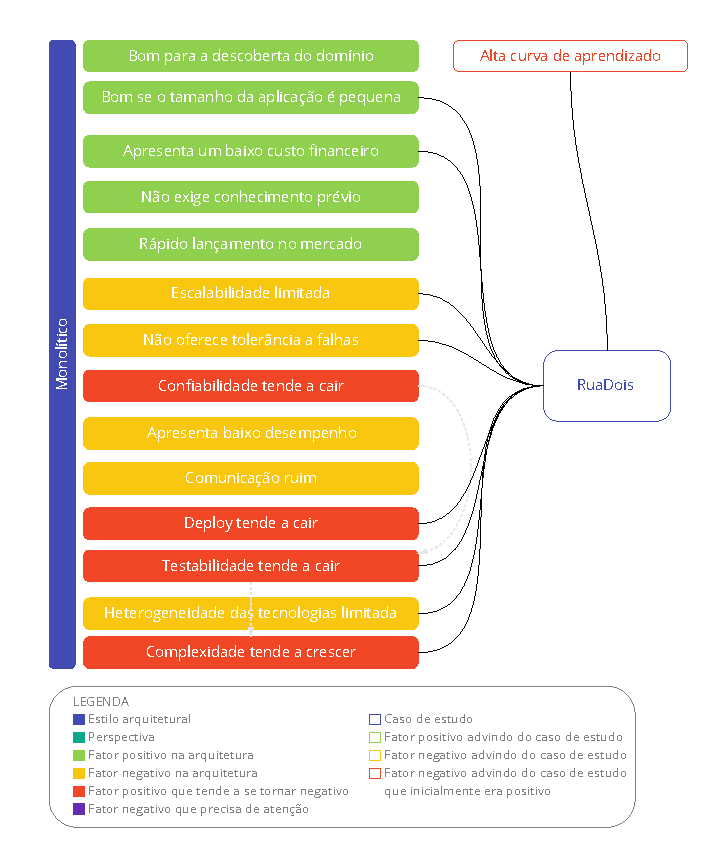
\includegraphics[keepaspectratio=true,scale=1]{figuras/analise-mono-ruadois.eps}
  \caption{Fatores apresentados no caso de estudo da arquitetura monolítica da RuaDois\label{fig:sintese-mono-ruadois}}
\end{figure}
